\apendice{Documentación de usuario}

\section{Introducción}

En este apéndice se van a mostrar los requisitos, la instalación y un manual para que el usuario final pueda manejar la aplicación de forma fluida. Para ello se ilustrará con figuras que muestren los detalles.

\section{Requisitos de usuarios}


\section{Instalación}

\section{Manual del usuario}

Una vez cumplamos los requisitos mínimos y hayamos instalado todo lo necesario, podremos comenzar a usar la aplicación. Lo primero que nos aparece al entrar en Thoth web es una ventana de inicio de sesión, como muestra la figura\ref{fig:6.1}.


\begin{figure}[h]
\centering
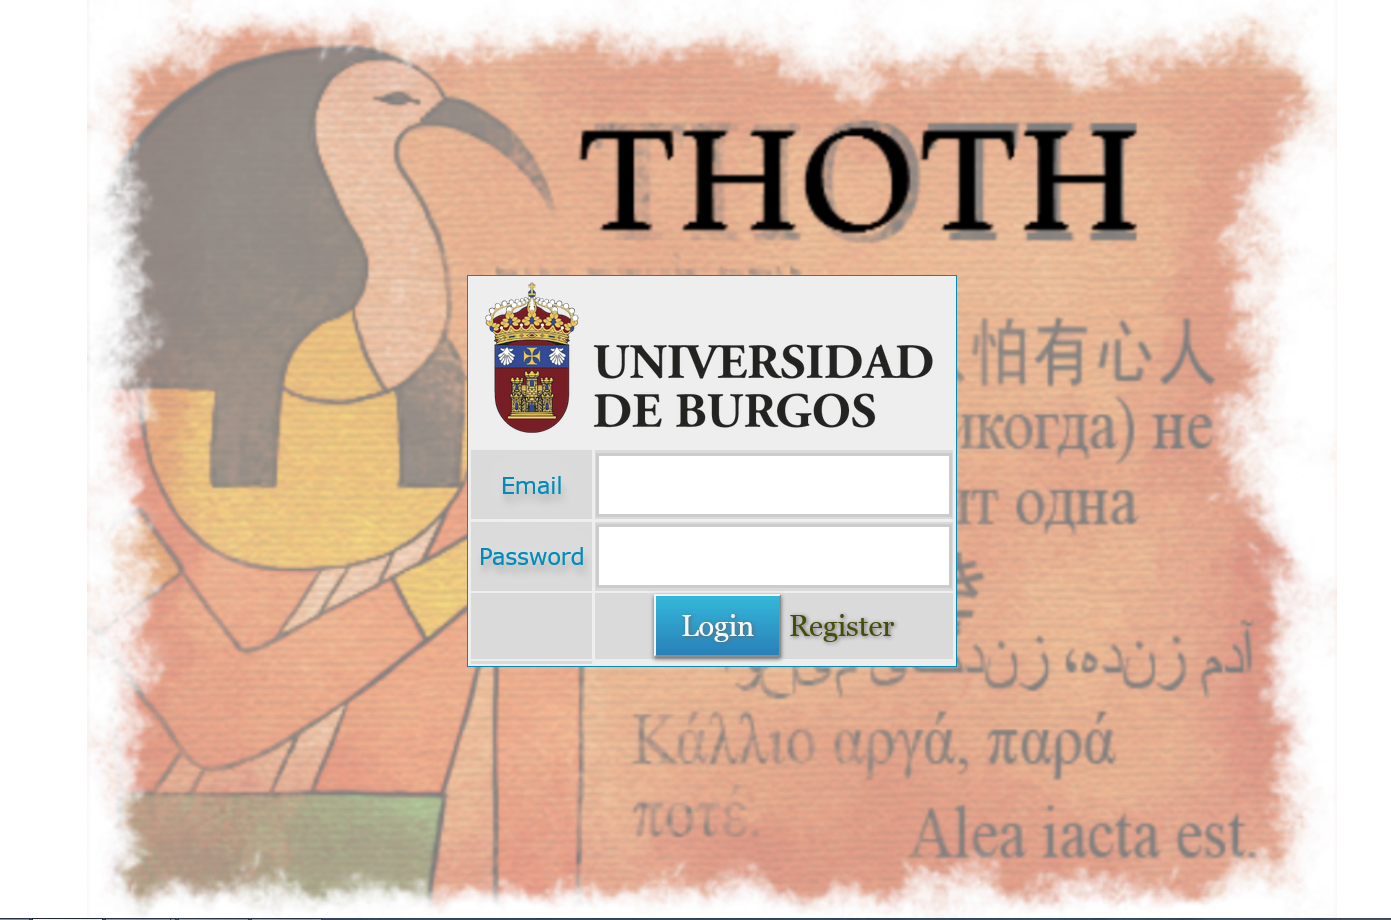
\includegraphics[width=0.50\textwidth]{Login}
\caption{Login en Thoth. Es lo que primero se ve al entrar en la aplicación.}
\label{fig:6.1}
\end{figure}

De inicio no tendremos creada una cuenta en Thoth, así que debemos registrarnos. Si pulsamos en <<Register>> aparecerá una vista con la siguiente pantalla\ref{fig:6.2}, en la que introducir los datos para crear una cuenta. Hay que tener en cuenta que los datos deben estar correctamente rellenados o de lo contrario, la aplicación nos mostrará un error. Si el fallo es el correo electrónico, se marcará el campo en rojo\ref{fig:6.3}. En el caso de que el registro haya sido correcto, se mostrara un mensaje indicativo.

\begin{figure}[h]
\centering
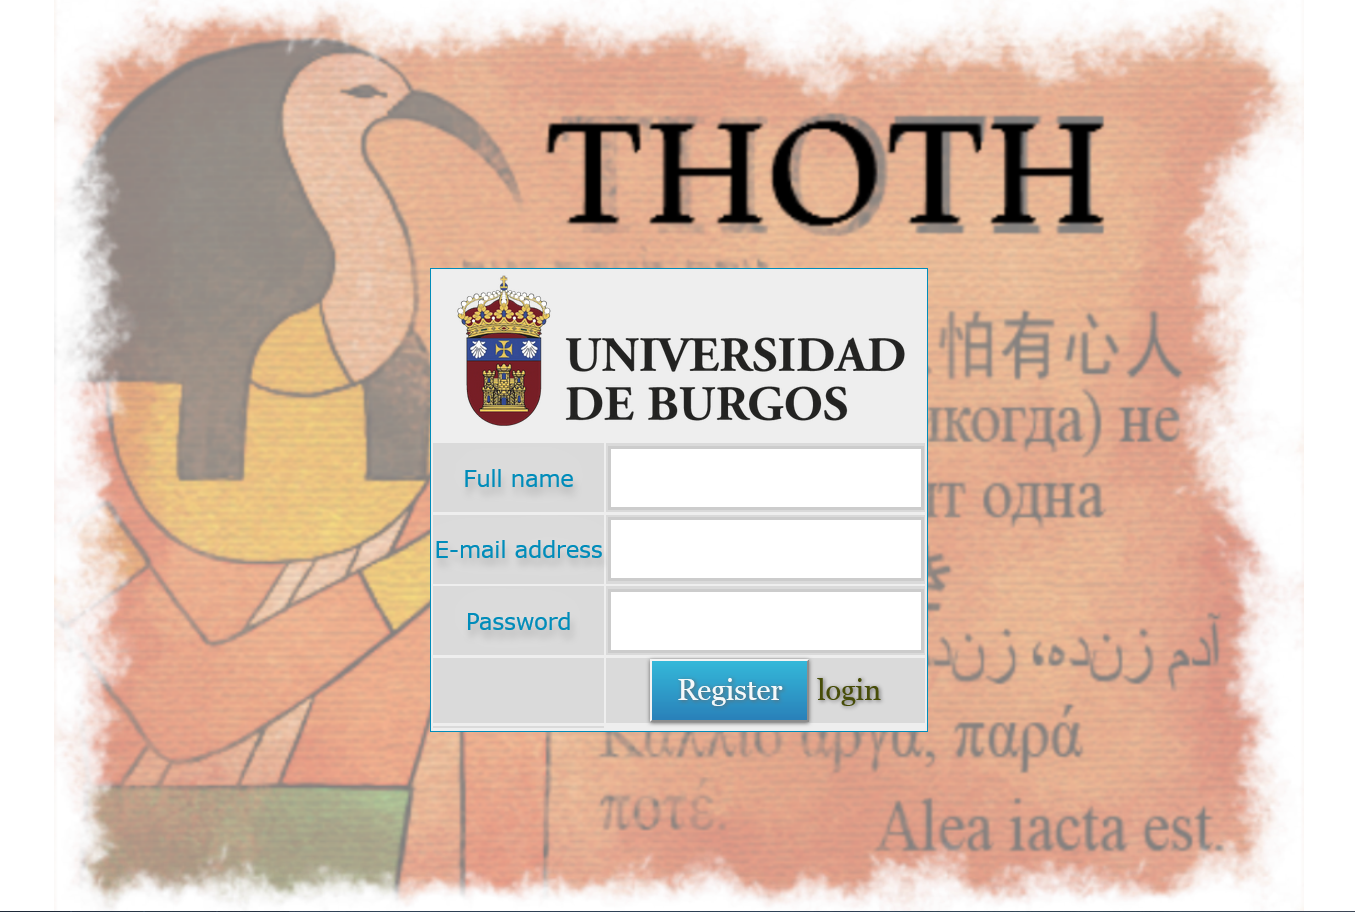
\includegraphics[width=0.50\textwidth]{Registro}
\caption{Pantalla de registro.}
\label{fig:6.2}
\end{figure}

\begin{figure}[h]
\centering
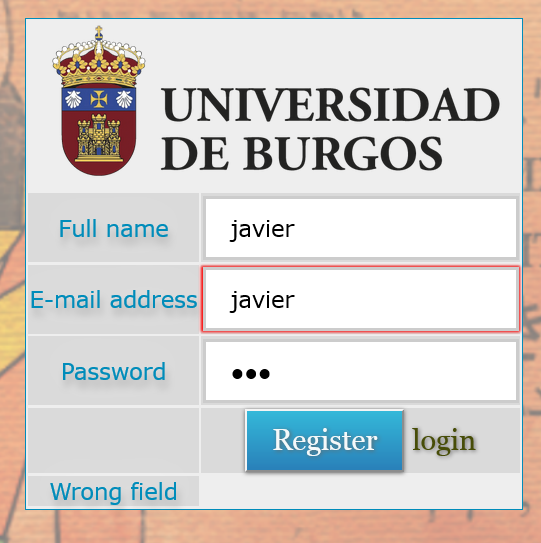
\includegraphics[width=0.40\textwidth]{Email-Error}
\caption{Fallo al introducir el email. Se muestra el campo en rojo.}
\label{fig:6.3}
\end{figure}

Una vez registrados, ahora sí, podremos iniciar sesión. Al hacerlo accedemos a la vista principal de la aplicación que consta de tres elementos principales. Un menú, en el que se despliegan diferentes opciones, un panel en el que introducir la gramática y por último una tabla con las características de la gramática. Esta vista se puede apreciar con detalle en la siguiente imagen \ref{fig:6.4}.


\begin{figure}[h]
\centering
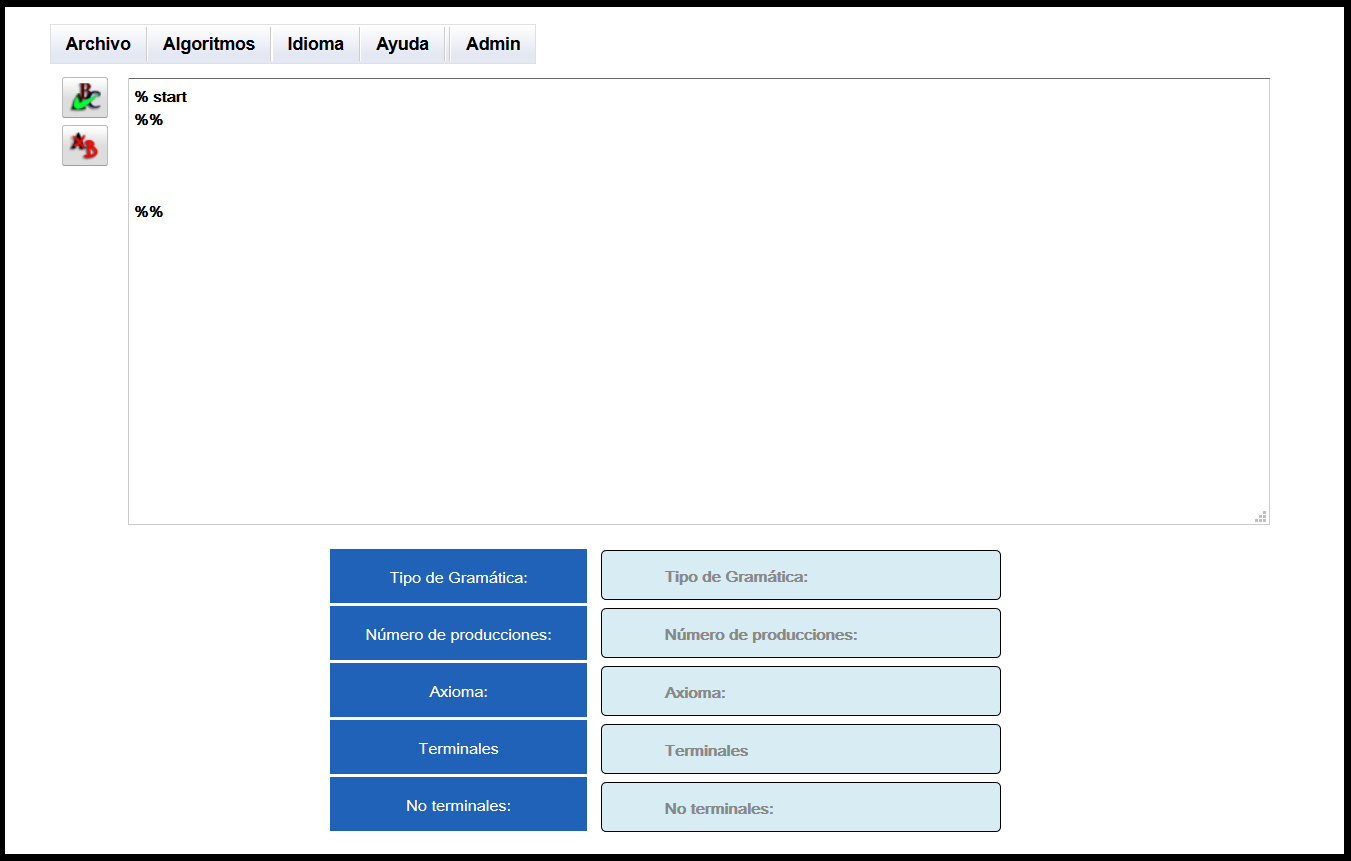
\includegraphics[width=1\textwidth]{Vista-Principal}
\caption{Pantalla principal con el menú de la aplicación y el panel para crear una gramática.}
\label{fig:6.4}
\end{figure}

Para empezar, podemos centrarnos en la introducción de la gramática. En el recuadro definido, podemos copiar, cortar, seleccionar y pegar texto. Para comprobar una gramática solo tenemos que pulsar el botón de <<checkear>> en la parte superior. Por otro lado si queremos buscar y reemplazar un símbolo, el botón de renombrado aparece debajo\ref{fig:6.5}. Para renombrar aparecerá una ventana con esta forma\ref{fig:6.6}.

\begin{figure}[h]
\centering

\includegraphics[width=0.30\textwidth]{botones-gramatica}
\caption{En la parte superior comprobar gramática y abajo renombrar.}
\label{fig:6.5}
\end{figure}

\begin{figure}[h]
\centering
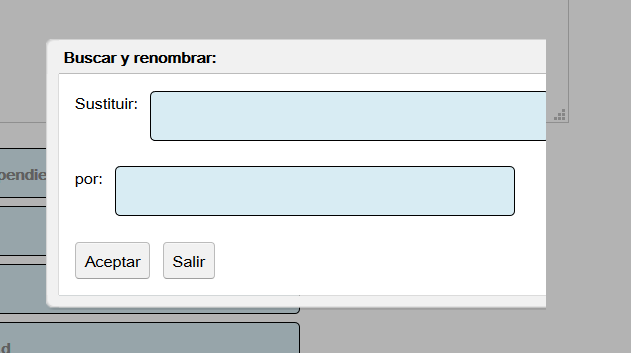
\includegraphics[width=0.40\textwidth]{Renombrado}
\caption{Renombrado de símbolos.}
\label{fig:6.6}
\end{figure}

Dentro de las opciones del menú, quizá la mas utilizada es la de elegir el algoritmo a aplicar a la gramática. En el desplegable se pueden ver todas las opciones que hay. Para no extendernos, mostraré las vistas de los algoritmos que sean diferentes a las demás. 

En primer lugar la siguiente imagen muestra el algoritmo de eliminación de símbolos anulables\ref{fig:6.7}. Es igual en la mayoría de los algoritmos. Se puede apreciar como se resaltan las producciones en color verde y otras en rojo. Esto sólo ocurre cuando se aplica el algoritmo paso a paso. De lo contrario, no mostrará el proceso, y simplemente aparecerá a un lado la gramática antigua y al otro la nueva.

\begin{figure}[h]
\centering
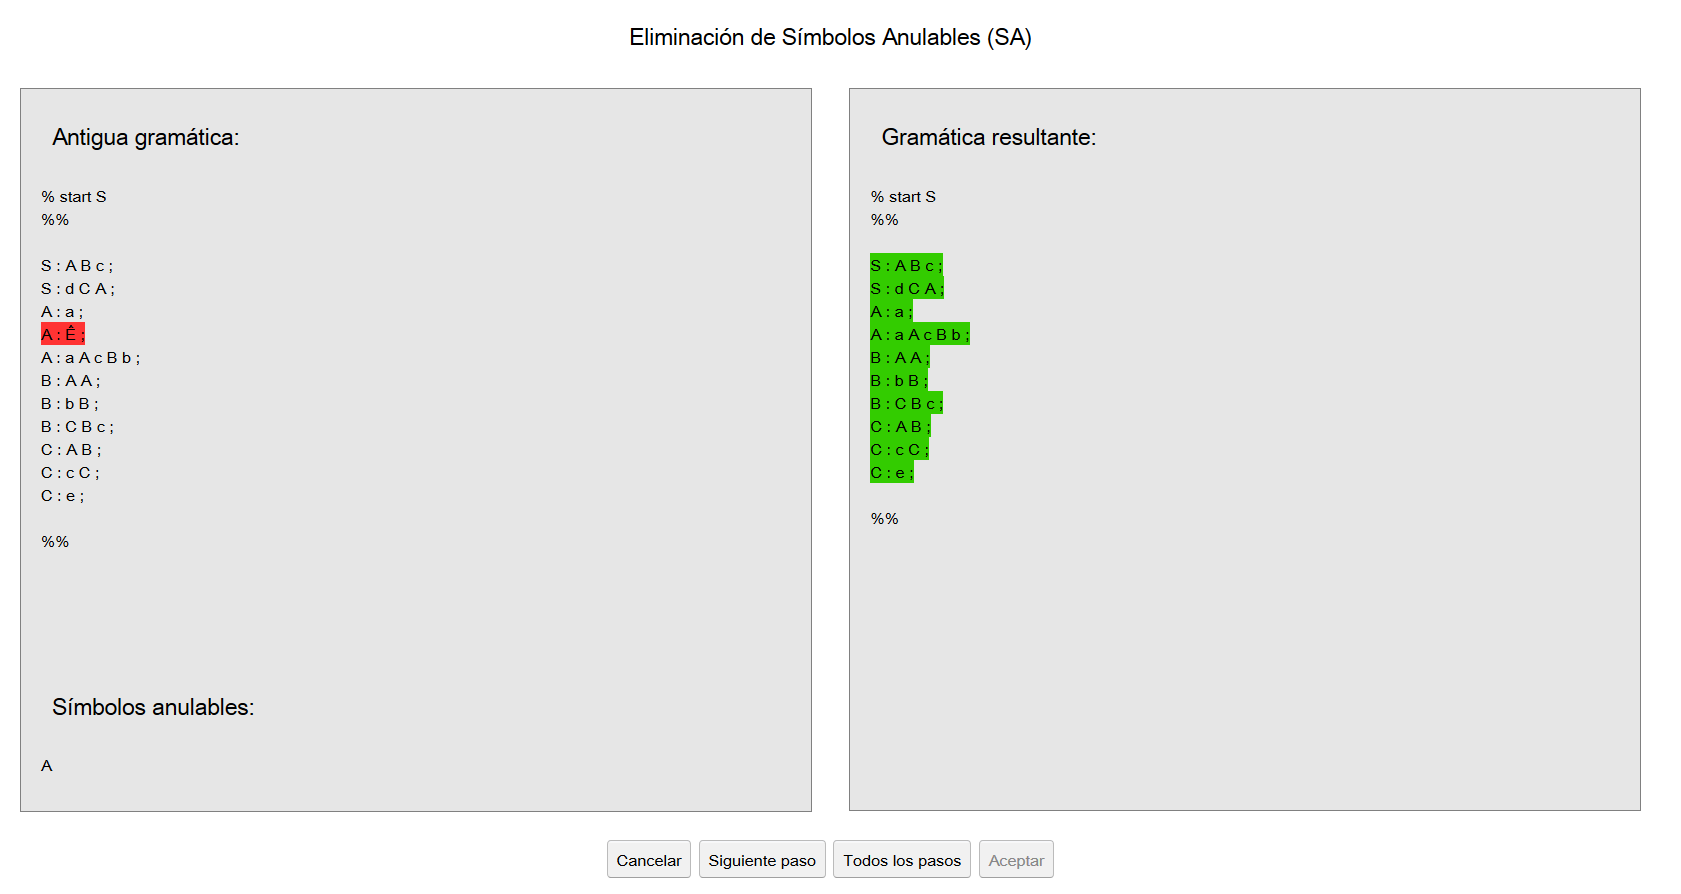
\includegraphics[width=1\textwidth]{vista-algoritmos}
\caption{Ejemplo de una vista del algoritmo Eliminación de SA.}
\label{fig:6.7}
\end{figure}

En verde se iluminan las producciones que pasan a la nueva gramática en ese paso, y en rojo se resalta el símbolo anulable que se está analizando.

El cálculo del First y el Follow y el reconocimiento por medio de TASP, son algoritmos con vistas algo diferentes a las anteriores. el cálculo FF deriva incluso al reconocimiento con TASP, ya que ambos son algoritmos de análisis ascendente. En el ejemplo de First-Follow con cada botón se crea la tabla correspondiente\ref{fig:6.8}. Los botones de desactivan a mediada que se utilizan.

\begin{figure}[h]
\centering
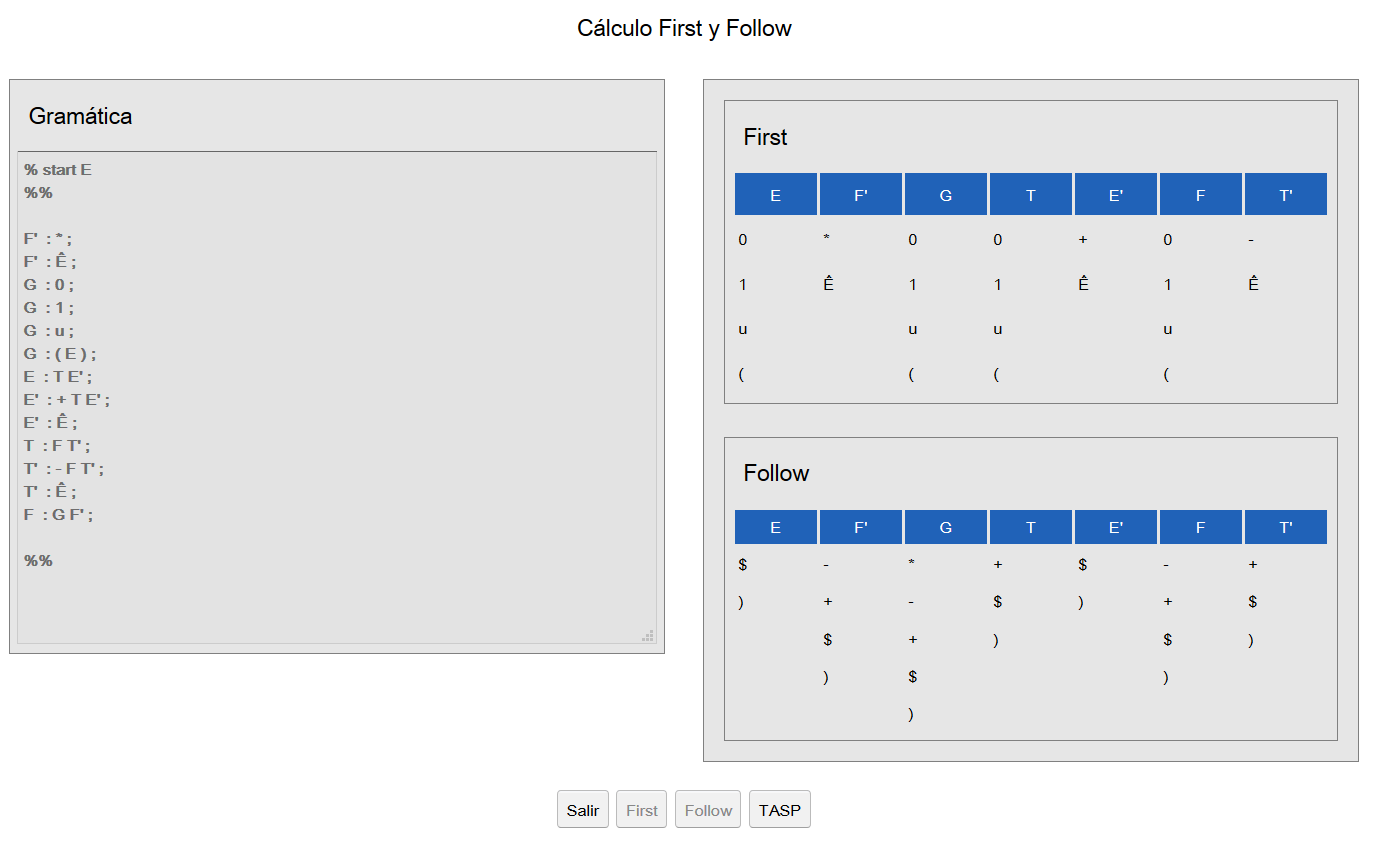
\includegraphics[width=1\textwidth]{calculo-ff}
\caption{Vista del algoritmo para el Cálculo de Fisrt Follow.}
\label{fig:6.8}
\end{figure}

Para el reconocimiento con TASP, se muestra las Tabla de Análisis Sintáctico Predictivo (TASP) y aparece un recuadro en el que introducir la palabra a analizar\ref{fig:6.9}. Verificamos que es la palabra que queremos, o podemos borrarla con con los dos botones que aparecen a su lado. A continuación se crea la traza según la opción que deseemos. Paso a paso o todos los pasos a la vez. Al terminar de calcular la traza se mostrará un mensaje advirtiendo si se ha reconocido o no la palabra.

\begin{figure}[h]
\centering
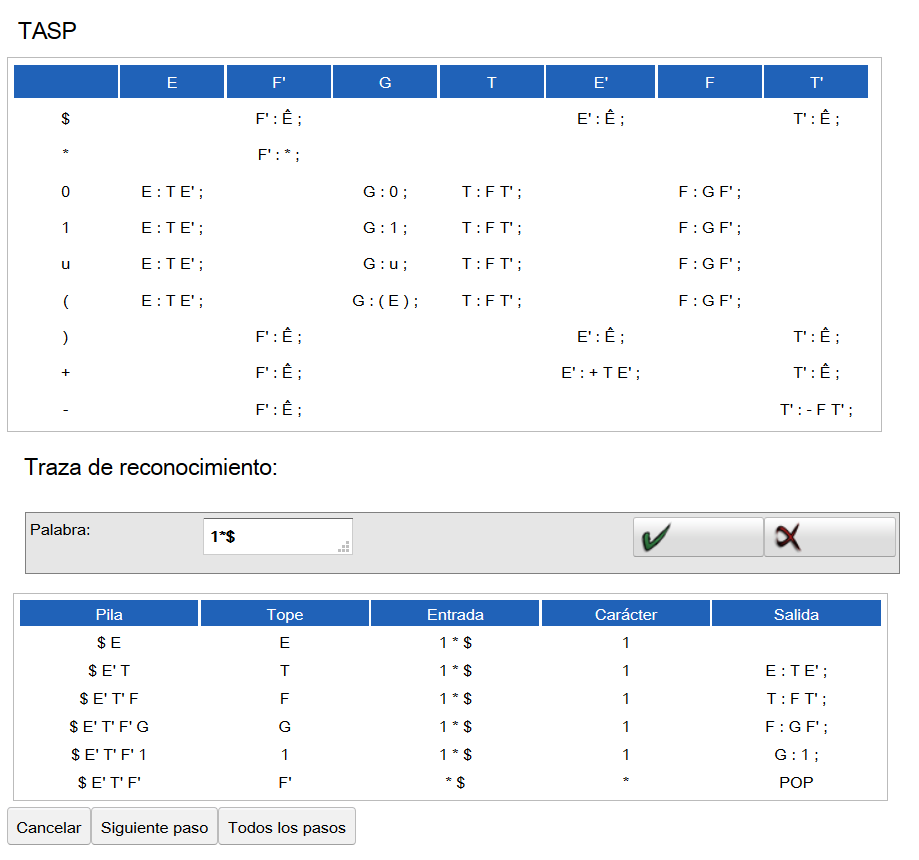
\includegraphics[width=1\textwidth]{reconocimiento-Tasp}
\caption{Vista del reconocimiento con TASP. Se aprecia la zona donde introducir la palabra y los botones.}
\label{fig:6.9}
\end{figure}

Volviendo al menú podemos apreciar que en las opciones aparece el nombre con el que se ha registrado el usuario. Si pulsamos en ello podremos ver como se despliega la opción para cerrar la sesión. Que aparezca en nombre da la seguridad de que nos encontramos en nuestra sesión, además de dar personalidad. Al cerrar sesión se volverá a la vista de <<login>> y deberemos acceder de nuevo escribiendo el correo y la contraseña.

\begin{figure}[h]
\centering
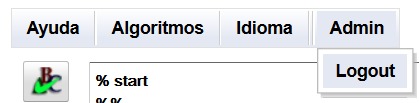
\includegraphics[width=0.40\textwidth]{menu-usuario}
\caption{Menú con el nombre del usuario. El desplegable muestra el cierre de la sesión.}
\label{fig:6.8}
\end{figure}

Siguiendo con el menú, la opción del idioma permite cambiar los textos de la aplicación, al idioma elegido. Como la vista se va a reiniciar y la gramática desaparecerá, es necesario mostrar un mensaje que solicita confirmación adicional.

\begin{figure}[h]
\centering
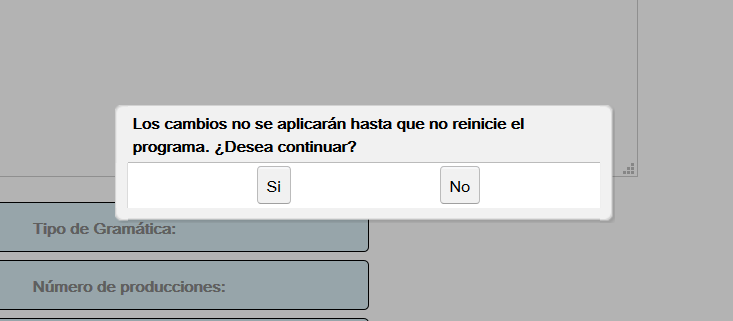
\includegraphics[width=0.40\textwidth]{opcion-idioma}
\caption{Mensaje de confirmación para cambiar el idioma.}
\label{fig:6.9}
\end{figure}

